\documentclass{article}
% WIP!
% Based upon: https://glennjlea.com/latex/creating-custom-title-page/
% Circuits Docs: https://texdoc.org/serve/circuitikz/0
\usepackage{bootstrapcolors}
\usepackage{tikz}
\usetikzlibrary{arrows,shapes.gates.logic.US,shapes.gates.logic.IEC,calc}
\begin{document}
    \color{orange-400}
    \pagecolor{blue-800}
    \thispagestyle{empty}
    \begin{center}
        \tikzstyle{branch}=[fill,shape=circle,minimum size=3pt,inner sep=0pt]
        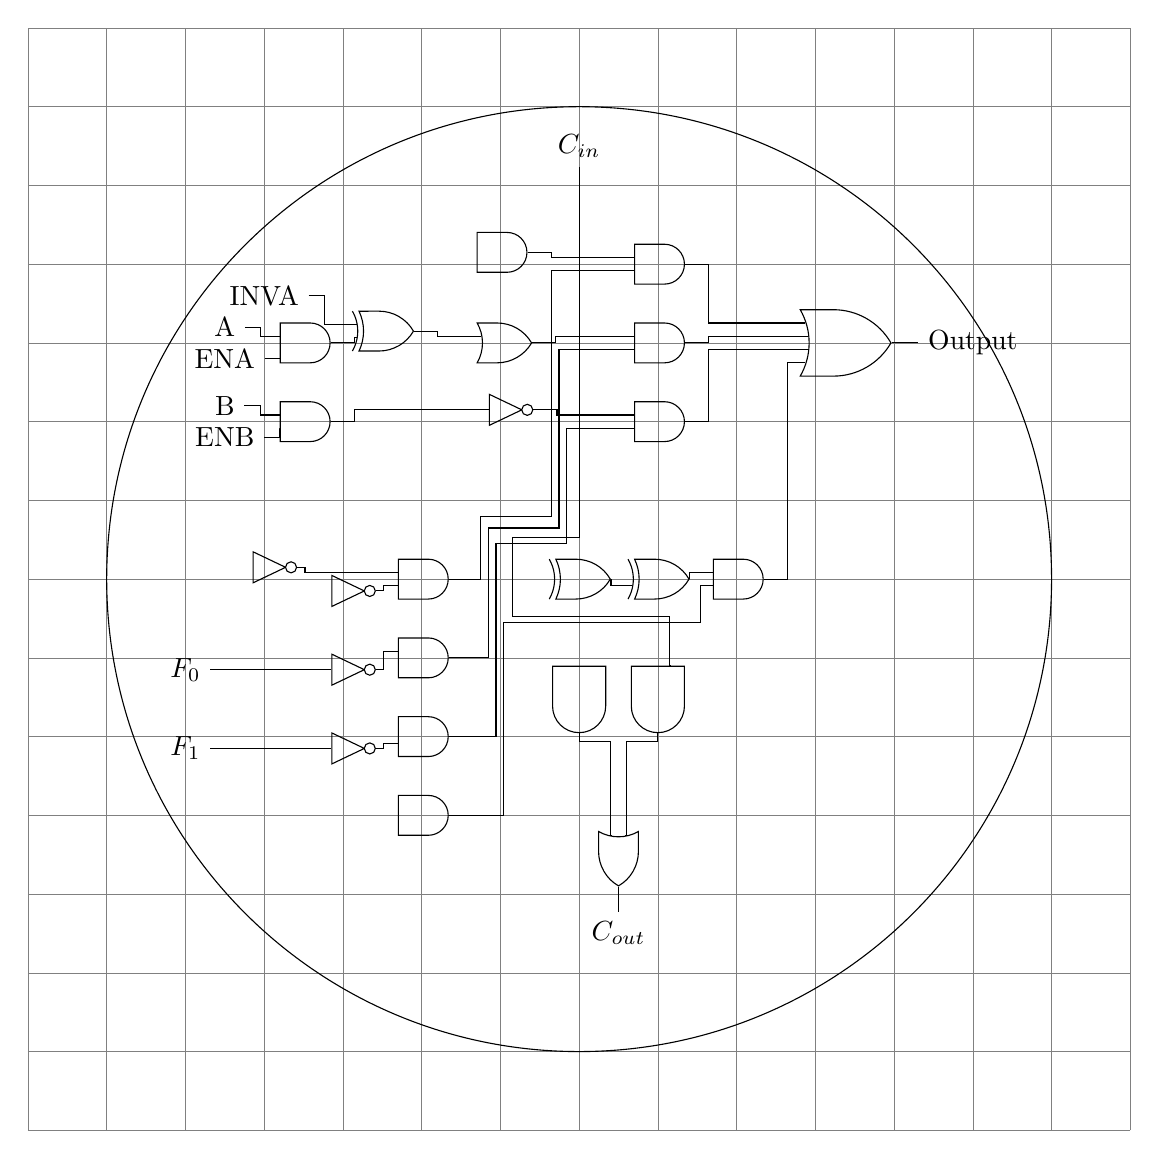
\begin{tikzpicture}
            % 1-bit ALU
            \draw[help lines] (-7,7) grid (7,-7); % Only for Development
            
            \node (inva) at (-4,3.6) {INVA};
            \node (a) at (-4.5,3.2) {A};
            \node (b) at (-4.5,2.2) {B};
            \node (ena) at (-4.5,2.8) {ENA};
            \node (enb) at (-4.5,1.8) {ENB};
            \node (f0) at (-5,-1.15) {$F_0$};
            \node (f1) at (-5,-2.15) {$F_1$};
            \node (cin) at (0,5.5) {$C_{in}$};
            \node (cout) at (0.5,-4.5) {$C_{out}$};
            \node (output) at (5,3) {Output};
            
            \node[and gate US, draw, logic gate inputs=nn] at (1,4) (AND1) {};
            \node[and gate US, draw, logic gate inputs=nn] at (1,3) (AND2) {};
            \node[and gate US, draw, logic gate inputs=nn] at (1,2) (AND3) {};
            
            \node[and gate US, draw, logic gate inputs=nn] at (-1,4.15) (AND4) {};
            \node[or gate US, draw, logic gate inputs=nn] at (-1,3) (OR1) {};
            \node[not gate US, draw, logic gate inputs=n] at (-1,2.15) (NOT1) {};
            
            \node[xor gate US, draw, logic gate inputs=nn] at (-2.5,3.15) (XOR1) {};
            \node[and gate US, draw, logic gate inputs=nn] at (-3.5,3) (AND5) {};
            \node[and gate US, draw, logic gate inputs=nn] at (-3.5,2) (AND6) {};
            
            \node[or gate US, draw, logic gate inputs=nnnn] at (3.3,3) (OR2) {};

            % left down
            \node[and gate US, draw, logic gate inputs=nn] at (-2,0) (AND7) {};
            \node[and gate US, draw, logic gate inputs=nn] at (-2,-1) (AND8) {};
            \node[and gate US, draw, logic gate inputs=nn] at (-2,-2) (AND9) {};
            \node[and gate US, draw, logic gate inputs=nn] at (-2,-3) (AND10) {};

            \node[not gate US, draw, logic gate inputs=n] at (-3,-0.15) (NOT2) {};
            \node[not gate US, draw, logic gate inputs=n] at (-3,-1.15) (NOT3) {};
            \node[not gate US, draw, logic gate inputs=n] at (-3,-2.15) (NOT4) {};
            
            \node[not gate US, draw, logic gate inputs=n] at (-4,0.15) (NOT5) {};
            %


            \node[xor gate US, draw, logic gate inputs=nn] at (0,0) (XOR2) {};
            \node[xor gate US, draw, logic gate inputs=nn] at (1,0) (XOR3) {};
            \node[and gate US, draw, logic gate inputs=nn] at (2,0) (AND11) {};
            
            \node[and gate US, draw, logic gate inputs=nnn,rotate=-90] at (0,-1.5) (AND12) {};
            \node[and gate US, draw, logic gate inputs=nnn,rotate=-90] at (1,-1.5) (AND13) {};
            \node[or gate US, draw, logic gate inputs=nn,rotate=-90] at (0.5,-3.5) (OR3) {};

            %\draw (a.south) -- ++(south:0mm) |- (GOR.input 1);
            %\draw (GOR.output) -- ++(right:3mm);
            \draw (AND1.output) -- ++(right:3mm) |- (OR2.input 1);
            \draw (AND2.output) -- ++(right:3mm) |- (OR2.input 2);
            \draw (AND3.output) -- ++(right:3mm) |- (OR2.input 3);
            \draw (AND11.output) -- ++(right:3mm) |- (OR2.input 4);

            \draw (AND12.output) -- ++(south:1mm) |- ++(east:4mm) |- (OR3.input 2);
            \draw (AND13.output) -- ++(south:1mm) |- ++(west:4mm) |- (OR3.input 1);
            
            \draw (AND7.output) -- ++(east:4mm) |- ++(north:8mm) |- ++(east:9mm) |- (AND1.input 2);
            \draw (AND8.output) -- ++(east:5mm) |- ++(north:16.5mm) |- ++(east:9mm) |- (AND2.input 2);
            \draw (AND9.output) -- ++(east:6mm) |- ++(north:24.5mm) |- ++(east:9mm) |- (AND3.input 2);
            \draw (AND10.output) -- ++(east:7mm) |- ++(north:24.5mm) |- ++(east:25mm) |- (AND11.input 2);

            \draw (AND4.output) -- ++(right:3mm) |- (AND1.input 1);
            \draw (OR1.output) -- ++(right:3mm) |- (AND2.input 1);
            \draw (NOT1.output) -- ++(right:3mm) |- (AND3.input 1);

            \draw (XOR3.output) -- ++(right:0mm) |- (AND11.input 1);
            \draw (XOR2.output) -- ++(right:0mm) |- (XOR3.input 2);
            
            \draw (NOT5.output) -- ++(right:1mm) |- (AND7.input 1);
            \draw (NOT2.output) -- ++(right:1mm) |- (AND7.input 2);
            \draw (NOT3.output) -- ++(right:1mm) |- (AND8.input 1);
            \draw (NOT4.output) -- ++(right:1mm) |- (AND9.input 2);

            %
            \draw (OR2.output) -- ++(right:3mm) |- (output.west);
            \draw (OR3.output) -- ++(south:3mm) |- (cout.north);
            
            \draw (a.east) -- ++(right:2mm) |- (AND5.input 1);
            \draw (ena.east) -- ++(right:2mm) |- (AND5.input 2);
            
            \draw (b.east) -- ++(right:2mm) |- (AND6.input 1);
            \draw (enb.east) -- ++(right:2mm) |- (AND6.input 2);
            
            \draw (f0.east) -- ++(right:2mm) |- (NOT3.input);
            \draw (f1.east) -- ++(right:2mm) |- (NOT4.input);
            
            \draw (inva.east) -- ++(right:2mm) |- (XOR1.input 1);

            \draw (cin.south) -- ++(south:47mm) |- ++(west:8.5mm) |- ++(south:10mm) |- ++(east:20mm) |- (AND13.input 1);
            
            \draw (AND5.output) -- ++(east:3mm) |- (XOR1.input 2);
            \draw (AND6.output) -- ++(east:3mm) |- (NOT1.input);

            \draw (XOR1.output) -- ++(east:3mm) |- (OR1.input 1);

            \draw (0,0) circle [radius=6];
        \end{tikzpicture}
    \end{center}
\end{document}